\documentclass[10pt]{article}
\usepackage{amsmath}
\usepackage{amssymb}
\usepackage[dvips]{graphicx}
\usepackage[small,bf]{caption}
\usepackage[american]{varioref}
\usepackage{fancyheadings}
\usepackage{wrapfig}
\usepackage{html}
\usepackage{color}

% Margin adjustments.  vmargin.sty interacts badly with page numbers at
% the bottom of the page, so we just code the number manually here.

\oddsidemargin  0pt
\evensidemargin 0pt
\topmargin      0pt
\hoffset        0 in
\textwidth      6.5 in
\textheight     9 in

% Style adjustments.

% Fix placement of figures & tables.  This keeps latex from shoving big
% floats to the end of a document when they are somewhat big, which it will
% do even if you put [htb] as the argument.

\setcounter{topnumber}{1}
\setcounter{bottomnumber}{1}
\def\topfraction{1.0}
\def\bottomfraction{1.0}
\def\textfraction{0.0}
\def\floatpagefraction{0.9}

%begin{latexonly}

\raggedbottom

\def\captionfont{\itshape}              % Use italic font for captions.

\makeatletter

\setlength{\parindent}{0 pt}            % Unindented paragraphs, separated ...
\setlength{\parskip}{1.3 ex}            % ... by roughly one blank line.

\renewcommand{\section}{\@startsection%
  {section}{1}{0pt}{-1.8ex \@plus -1ex \@minus -.2ex}%
  {0.8ex}{\normalfont\Large\bfseries}}

\renewcommand{\subsection}{\@startsection%
  {subsection}{2}{0pt}{-2ex \@plus 1ex \@minus -.2ex}%
  {0.8ex}{\slshape\large\bfseries}}

\renewcommand{\subsubsection}{\@startsection%
  {subsubsection}{3}{0pt}{-1.5ex \@plus 1ex \@minus -.2ex}%
  {0.5ex}{\slshape\normalsize\bfseries}}

\newcommand{\tightspacing}{\renewcommand{\baselinestretch}{0.85}}
\newcommand{\regularspacing}{\renewcommand{\baselinestretch}{1.0}}

\makeatother

% Page footings.

\pagestyle{fancy}
\setlength{\headrulewidth}{0 pt}
\lhead{} \chead{} \rhead{}
% \lfoot{\emph{Internal design document}}
% \rfoot{\emph{Do not quote or redistribute}}

%end{latexonly}

% Miscellaneous macros.

\newcommand{\boxedgraphic}[2][]{\def\fboxsep{0pt}\fbox{\includegraphics[#1]{#2}}}
\newcommand{\url}[1]{\textup{\texttt{#1}}}
\newcommand{\menu}[1]{\textsf{\textbf{#1}}}
\newcommand{\class}[1]{\textsf{#1}}
\newcommand{\attrib}[1]{\textsf{#1}}
\newcommand{\attribtype}[1]{\textsf{#1}}

\newcommand{\notationdocloc}{\url{ftp://ftp.cds.caltech.edu/pub/caltech-erato/notation/}}
\newcommand{\eratowebloc}{\url{http://www.cds.caltech.edu/erato/}}

\begin{document}

%=============================================================================
% Title page
%=============================================================================

\thispagestyle{fancy}

\title{\textbf{An XML-Based Model Description Language\\
    for Systems Biology Simulations}}

\author{Michael Hucka, Herbert Sauro, Andrew Finney, Hamid Bolouri\\
\normalsize\texttt{\{mhucka,hsauro,afinney,hbolouri\}@cds.caltech.edu}\\[-2pt]
\normalsize ERATO Kitano Systems Biology Project\\[-2pt]
\normalsize Control and Dynamical Systems 107-81\\[-2pt]
\normalsize California Institute of Technology, Pasadena, CA 91125\\[10pt]
\normalsize This document is based on discussions with the authors of\\[-2pt]
\normalsize BioSpice (Arkin), DBSolve (Goryanin), E-Cell (Tomita, Nakayama, Takahashi),\\[-2pt]
\normalsize Gepasi (Mendez), StochSim (Bray, Firth \& Shimizu), Virtual Cell (Loew \& Schaff),\\[-2pt]
\normalsize and the ERATO Kitano Systems Biology Project group.}

\date{\today{}}

\maketitle

\thispagestyle{fancy}

\vspace*{0.5 in}


%=============================================================================
\section{Introduction} 
\label{sec:introduction}
%=============================================================================

We present a first attempt at specifying a common, model-based description
language for systems biology simulation software.  The overall goal is to
develop a common language that will enable simulation software to
communicate and exchange models, ultimately leading to the ability for
researchers to run simulations and analyses across multiple software
packages.

The model-based description language presented here is the result of
merging the most obvious modeling-language features of BioSpice, E-Cell,
Gepasi, DBSolve, StochSim, and Virtual Cell.  Along with the description
language, we also describe how instances of data structures can be encoded
in XML, the Extensible Markup Language~(Bosak and Bray, 1999; Bray, Paoli
and Sperberg-McQueen, 1998).  However, the associated XML encoding is not
intended to be a complete file storage format.  This XML encoding of the
description language \emph{could} be extended to define a file format (for
example, by introducing additional components such as file headers);
however, at this time, we are focusing only on using the XML-based
description language as an interchange format for use in communications
between programs.

The primary purpose of this document is to serve as a basis for discussion
and further development of a more comprehensive language specification.
The final outcome of this process will be a collection of XML Schemas which
can be used to translate model descriptions between simulation packages.
Because XML Schemas are difficult to read and absorb by human readers, we
define the proposed data structures using a succinct graphical notation
based on a subset of UML, the Unified Modeling Language (Eriksson, 1998;
Oestereich, 1999).  Our notation is explained in \emph{A Notation for
  Describing Model Representations Intended for XML Encoding}~(Hucka,
2000), available online at \notationdocloc{}.  For the sake of clarity, we
ask readers to use this notation when contributing to discussions about the
specification.  To facilitate discussions, a web/FTP site and a group
mailing list have been set up for the seven participating groups.  Please
see the web site at \eratowebloc{} for details.


%=============================================================================
\section{Overview} 
\label{sec:overview}
%=============================================================================

The representation language is organized around five categories of
information: model, compartment, geometry, specie and reaction.  Not all of
these will be needed by every simulation package; rather, the intent is to
cover the range of data structures needed by the collection of all six
simulators examined so far.

\begin{figure}
  \centering
  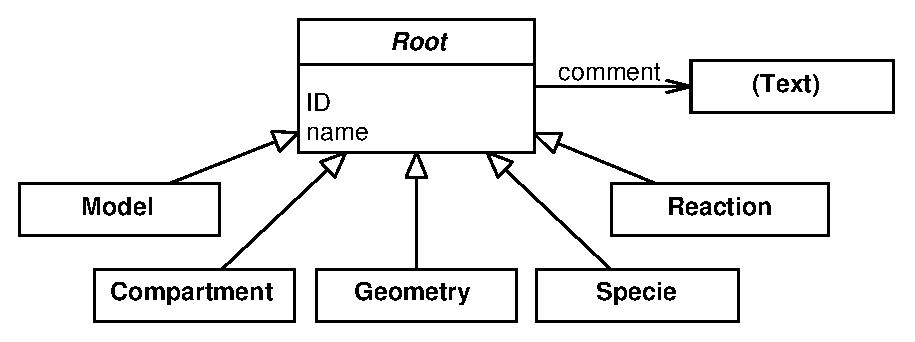
\includegraphics[scale = 0.75]{top-level.eps}
  \caption{A diagram of the highest level of the object class hierarchy.}
  \label{fig:top-level}
\end{figure}

Figure~\ref{fig:top-level} depicts the highest level of organization of the
objects in the model description language.  It shows that the main object
classes are derived from a \class{Root} class containing attributes
\attrib{ID}, \attrib{name}, and \attrib{comment}.  The five classes,
\class{Model}, \class{Compartment}, \class{Geometry}, \class{Species} and
\class{Reaction} all inherit these attributes.  The classes are described
in the next section.

This division of data structures into five categories, as well as the
particular names of the classes and the manner of specifying relations
between them, are fairly arbitrary and open to discussion.  The current
collection is intended to be parsimonious and unambiguous.

The present definition of the model description language does not include a
specification for units.  Units will have to be added to the final version,
and we expect that extending the representation language to include
information about units will be straightforward, but we await further
discussion with the user community on this matter.

The present state of the language also does not include specifications for
the data types of attributes.  The XML Schema presented in
Appendix~\ref{apdx:schemas} \emph{does} include preliminary type
specifications, but the chosen types are not necessarily final.  They are
provided mainly as illustrative examples.  Type specifications will be
included in the final definition of the language, after additional
discussions with the user community.  For the time being, we hope that most
attribute types described here are reasonably self-evident.  For example,
\attrib{name} attributes can be expected to be text strings, whereas
attributes such as \attrib{x}, \attrib{y} and \attrib{z} coordinates can be
expected to be floating point numbers.  The \attrib{ID} attribute in the
\class{Root} object is intended to be a unique numerical identifier
assigned to every instance of an object.

A few assumptions about the form of the language are not necessarily
self-evident.  In particular,
\begin{itemize}
  
\item We assume that, in order for each simulator program to read and write
  the model description language, they will require native interface code.
  This interface code will have to translate the simulator's internal data
  structures back and forth from the model description language.  We assume
  that this interface code will massage data structures as appropriate in
  order to smooth out small differences in conceptual organization between
  a simulator's specific internal representation and the model description
  language.

\item A zero value is not the same as an empty attribute value.  The model
  description language uses a number of structures that, in a given object
  instance, may be empty, depending on whether a given simulator needs
  them.  Programs that interpret objects expressed in the language must be
  designed to pay attention to this distinction.

\end{itemize}

%=============================================================================
\section{Elements of the Model Description Language}
\label{sec:elements}
%=============================================================================

In the following sections, we discuss in turn each of the five major object
classes that are subclasses of \class{Root} in the representational
hierarchy.


%-----------------------------------------------------------------------------
\subsection{Model}
%-----------------------------------------------------------------------------

The \class{Model} class defines a grouping of components.  There is only
one object of type \class{Model} per instance of a model description
language document or data stream, and it contains the list of compartments,
species and reactions that define a given model.  The UML-based definition
of the class is shown in Figure~\ref{fig:model}.

\begin{figure}[tb]
  \centering
  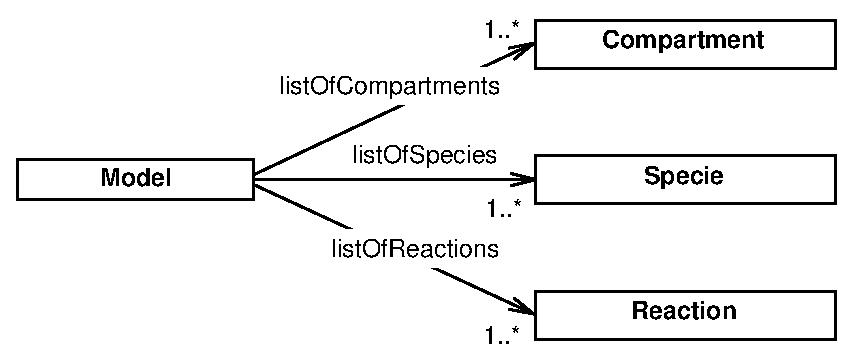
\includegraphics[scale = 0.75]{model.eps}
  \caption{A diagram of \class{Model}.  As shown in
    Figure~\ref{fig:top-level}, \class{Model} is a subclass of the
    \class{Root} object class, which means that \class{Model} implicitly
    inherits the attributes of \class{Root} (namely, \attrib{ID},
    \attrib{name} and \attrib{comment}).  The inherited attributes are not
    shown here.}
  \label{fig:model}
\end{figure}

The definition shows that there must be at least one specie, one reaction
and one compartment in a model; otherwise, there would be little point in
defining the model in the first place.  There is no restriction on the
total number of these elements.

%This definition shows that \class{Model} in this framework
%is a hierarchical grouping construct.  It does not have geometry or other
%characteristics itself; instead, the \class{Compartment} objects are the
%ones that hold geometries and other attributes.  Compartment objects are
%intented to be the leaf elements in a hierarchical tree, as shown in the
%following illustration, in which the top-most \class{Model}
%object contains two \class{Compartment} objects and another
%\class{Model} object:

%\begin{center}
%  \includegraphics{structure-tree.eps}
%\end{center}


%-----------------------------------------------------------------------------
\subsection{Compartments}
%-----------------------------------------------------------------------------

A \class{Compartment} object groups physical and geometrical
(morphological) details.  The definition of \class{Compartment} is shown in
Figure~\ref{fig:compartment}.

\begin{figure}[tb]
  \centering
  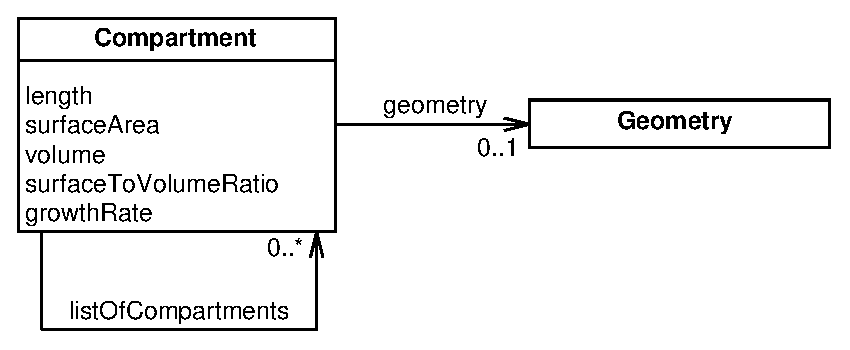
\includegraphics[scale = 0.75]{compartment.eps}
  \caption{The \class{Compartment} object class definition.}
  \label{fig:compartment}
\end{figure}

The dimensionality of a compartment can be one, two, or three dimensions,
and a given compartment can have an overall physical size; these aspects
are determined in an instance of a \class{Geometry} object by which of the
three size attributes are given a value: either \attrib{length} (for 1D),
\attrib{surfaceArea} (for 2D), or \attrib{volume} (for 3D).  Some examples
of different dimensionalities are: DNA stretch (1D); disks in
photoreceptors (2D); patch of membrane (2D); cell nucleus (3D); and
dendritic spines (3D).  The size of a compartment may change over the
course of a simulation.  The attribute \attrib{growthRate} can be used to
represent the rate at which the change in size takes place.  As its name
implies, the attribute \attrib{surfaceToVolumeRatio} records the
surface-to-volume ratio, a quantity that is of interest in some simulation
domains.

The geometric characteristics of a compartment are described using a
\class{Geometry} object.  The geometry information is optional, allowing
compartments to serve simply as topological structures if desired.  A
compartment may contain other compartments.  The subcompartments are listed
on the \attrib{listOfCompartments} attribute.  This allows nested
structures to be represented.  For example, a simple cell structure such as
that shown below,

\begin{center}
  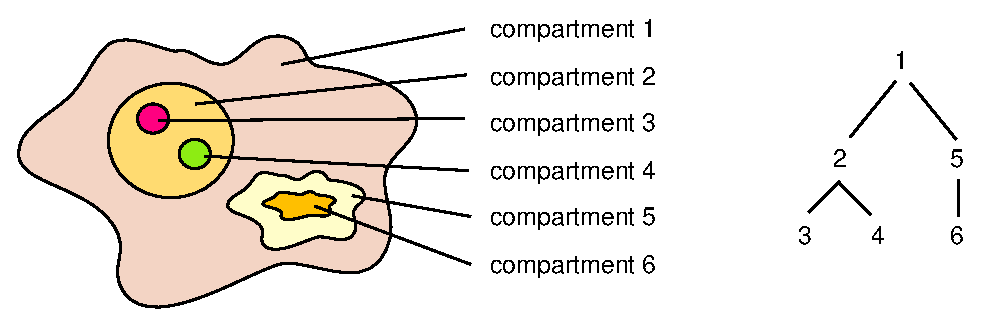
\includegraphics[scale = 0.75]{cell.eps}
\end{center}

would be described using one outer compartment containing two other
compartments, each of which contain more compartments themselves.


%-----------------------------------------------------------------------------
\subsection{Geometry}
%-----------------------------------------------------------------------------

A \class{Compartment} object can contain up to one \class{Geometry} object.
The \class{Geometry} class is intended to provide a means for specifying
morphological characteristics of compartments in simulations.  It is
defined in Figure~\ref{fig:geometry}.

\begin{figure}[hb]
  \centering
  \includegraphics[scale = 0.75]{geometry.eps}
  \caption{The \class{Geometry} object class definition.}
  \label{fig:geometry}
\end{figure}

The geometrical information is a boundary specification which can take the
form of either a list of algebraic functions, or a set of $(x,y,z)$
coordinates in a global reference frame.  The lists are contained by the
attributes \attrib{formulas} and \attrib{coordinates}, respectively.  As an
example of how the two forms might be used, consider a disk: it could be
expressed in algebraic form as $x^2 + y^2 <= r^2$, or it could be expressed
as a set ${(x,y,z)}$ of points on the boundary.


%-----------------------------------------------------------------------------
\subsection{Species}
%-----------------------------------------------------------------------------

``Species'' comprise all entities which take part in reactions.  The
\class{Specie} class is intended to represent these entities.  These
include simple ions (e.g., protons, calcium, etc.), simple molecules (e.g.,
glucose, ATP, etc.), and large molecules (e.g., RNA, polysaccharides, and
proteins).  Figure~\ref{fig:specie} presents the definition of
\class{Specie}.

\begin{figure}
  \centering
  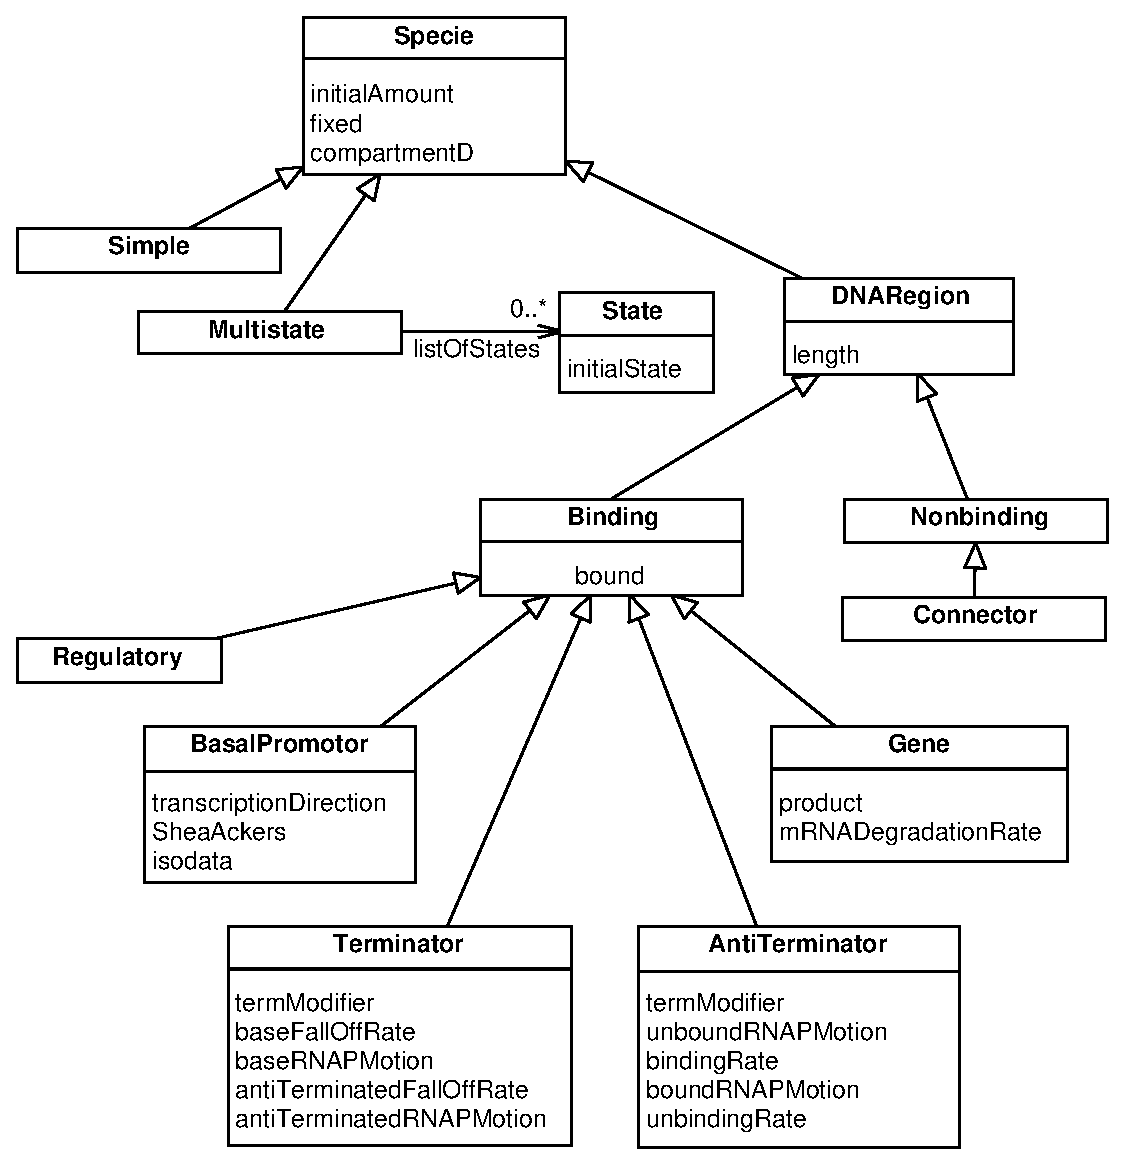
\includegraphics[scale = 0.75]{specie.eps}
  \caption{The \class{Specie} object class definition.}
  \label{fig:specie}
\end{figure}

Subclasses of \class{Specie} are divided into \class{Simple},
\class{Multistate}, and \class{DNARegion}, according to the types of
reactions they take part in.  ``Simple'' and ``multistate'' species are
self-explanatory.  Although ``multistate'' species could in principle be
defined as multiple \class{Simple} species, they are defined separately to
accommodate StochSim's method of simulating multistate receptors.

``DNA Region'' species are currently employed in a simple way in E-Cell,
and more comprehensively in BioSpice/Simulac for models of transcriptional
control.  The definition here is essentially that used in BioSpice/Simulac.
The \class{DNARegion} class has subclasses \class{Binding} and
\class{Nonbinding}, corresponding to the notion of ``binding'' and
``nonbinding'' DNA regions, respectively.  Binding regions are then divided
into various functional types such as \class{Regulatory}, \class{Promoter},
\class{Coding} (GENE), \class{Terminator} and \class{AntiTerminator}
regions.  Each of these subregions is given a set of attributes specific to
its role in transcription.

The attribute \attrib{initialAmount} is used to set the initial amount of
the specie.  The attribute \attrib{fixed} is a boolean value that
determines whether the amount of the specie is fixed or variable over the
course of a simulation.  The attribute \attrib{compartment} is used to
identify the compartment in which the specie belongs.


%-----------------------------------------------------------------------------
\subsection{Reactions}
%-----------------------------------------------------------------------------

In this framework, reactions are defined using lists of reactant species,
products, and their stoichiometries, and by parameter values for
separately-defined kinetic laws.  Three main types of reactions are
defined: simple, multistate, and DNA region, using the subclasses
\class{SimpleReaction}, \class{MultistateReaction} and
\class{DNARegionReaction}, respectively.  Multistate reactions are defined
separately in order to allow dynamically variable reaction rates and
transport between compartments.  DNA Region reactions are different from
the other two reaction types to allow different levels of abstraction in
modeling transcriptional control (e.g., stochastic and logical
interactions).  Figure~\ref{fig:reaction} presents the definition of the
\class{Reaction} object class.

\begin{figure}
  \centering
  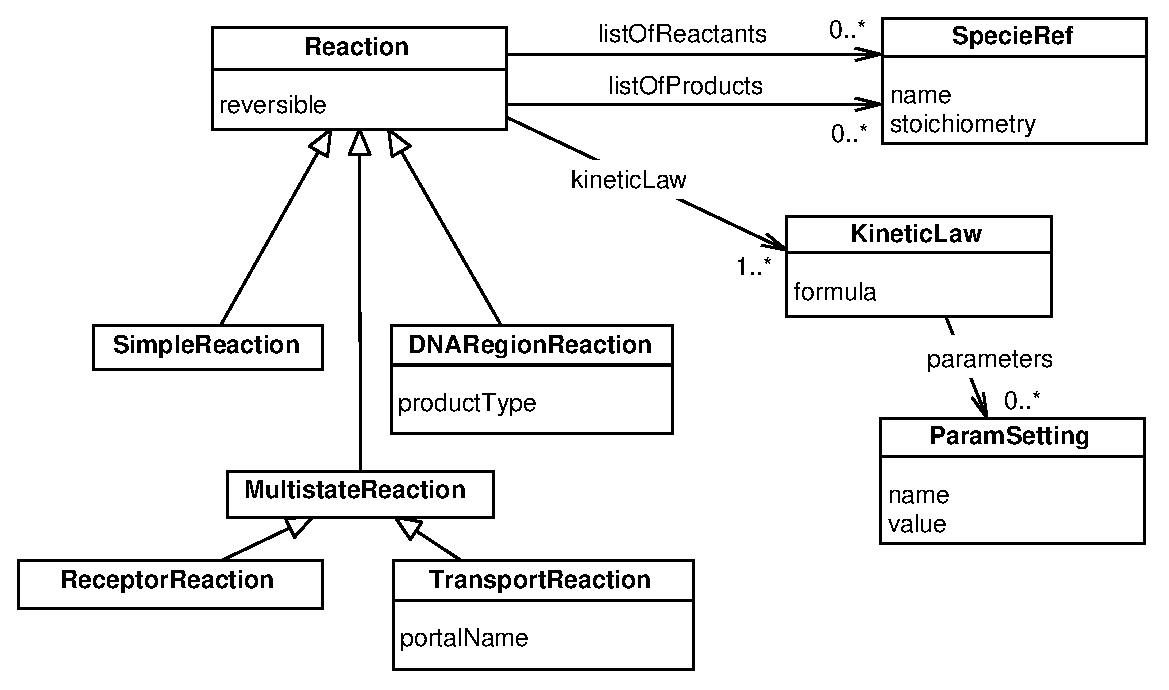
\includegraphics[scale = 0.75]{reaction.eps}
  \caption{The \class{Reaction} object class definition.}
  \label{fig:reaction}
\end{figure}

The attribute \attrib{name} in the \class{SpecieRef} substructure in
Figure~\ref{fig:reaction} is intended to refer to the name of a specie in
the species list of the model.  In other words, the species involved in a
reaction are listed once in a model, in the compartment, and the
\attrib{listOfReactants} and \attrib{listOfProducts} in reactions refer to
the list of species.

The example in the next section clarifies how the elements of the
\class{Reaction} class are intended to be used.


%=============================================================================
\section{Using the XML Encoding of the Model Description Language}
\label{sec:xml-rep}
%=============================================================================

In this section, we present an example of translating a model into the
systems biology model description language defined in this document.  The
approach to translating into XML the object class definitions presented in
the sections above is described in the companion document \emph{A
  Notation for Describing Model Representations Intended for XML
  Encoding}~(Hucka, 2000).  Appendix~\ref{apdx:schemas} gives the full
listing of a preliminary version of an XML Schema corresponding to the
systems biology model description language.

%-----------------------------------------------------------------------------
\subsection{Example Application of the Model Description Language}
%-----------------------------------------------------------------------------

The following example is the main portion of an XML document that describes
a simple branch system of the following form:
\[
\begin{array}{ccc}
& {k1 * X0}\\
X0 & \longrightarrow & S1
\end{array}
\]
\[
\begin{array}{ccc}
& {k2 * S1}\\
S1 & \longrightarrow & X1
\end{array}
\]
\[
\begin{array}{ccc}
& {k3 * S1}\\
S1 & \longrightarrow & X2
\end{array}
\]

\begin{figure}
  \small
  \tightspacing
\begin{verbatim}
<sbml>
  <Model id="1" name="Branch">
    <comment>Simple branch system.  The reaction looks like this:
                 reaction-1:   X0 -> S1; k1*X0;
                 reaction-2:   S1 -> X1; k2*S1;
                 reaction-3:   S1 -> X2; k3*S1;
    </comment>

    <listOfCompartments>
      <Compartment id="1" name="compartmentOne" volume="1"/>
    </listOfCompartments>

    <listOfSpecies>
      <Specie type="Simple" id="1" name="S1" initialAmount="0" fixed="no"  compartmentID="1"/>
      <Specie type="Simple" id="2" name="X0" initialAmount="0" fixed="yes" compartmentID="1"/>
      <Specie type="Simple" id="3" name="X1" initialAmount="0" fixed="yes" compartmentID="1"/>
      <Specie type="Simple" id="4" name="X2" initialAmount="0" fixed="yes" compartmentID="1"/>
    </listOfSpecies>

    <listOfReactions>
      <Reaction type="SimpleReaction" id="1" name="reaction_1" reversible="no">
        <listOfReactants>
          <SpecieRef name="X0" stoichiometry="1"/>
        </listOfReactants>
        <listOfProducts>
          <SpecieRef name="S1" stoichiometry="1"/>
        </listOfProducts>
        <kineticLaw formula="k1*X0">
          <listOfParameters>
            <ParamSetting name="k1" value="0"/>
          </listOfParameters>
        </kineticLaw>
      </Reaction>
      <Reaction type="SimpleReaction" id="2" name="reaction_2" reversible="no">
        <listOfReactants>
          <SpecieRef name="S1" stoichiometry="1"/>
        </listOfReactants>
        <listOfProducts>
          <SpecieRef name="X1" stoichiometry="1"/>
        </listOfProducts>
        <kineticLaw formula="k2*S1">
          <listOfParameters>
            <ParamSetting name="k2" value="0"/>
          </listOfParameters>
        </kineticLaw>
      </Reaction>
      <Reaction type="SimpleReaction" id="3" name="reaction_3" reversible="no">
        <listOfReactants>
          <SpecieRef name="S1" stoichiometry="1"/>
        </listOfReactants>
        <listOfProducts>
          <SpecieRef name="X2" stoichiometry="1"/>
        </listOfProducts>
        <kineticLaw formula="k3*S1">
          <listOfParameters>
            <ParamSetting name="k3" value="0"/>
          </listOfParameters>
        </kineticLaw>
      </SimpleReaction>
    </listOfReactions>
  </Model>
</sbml>
\end{verbatim}
  \tightspacing
  \caption{XML encoding of a simple example reaction.}
  \label{fig:simple-xml-example}
\end{figure}

The corresponding XML encoding shown in Figure~\ref{fig:simple-xml-example}
is quite straightforward.  The outermost container is a tag, \texttt{smbl},
that identifies the contents as being \underline{s}ystems \underline{b}iology
\underline{m}arkup \underline{l}anguage, an application of XML.  The next-inner
container is a single \texttt{Model} object which serves as the
highest-level object in the model.  The model in this case contains a
single \texttt{Compartment} object.

The compartment has four species associated with it, and three reactions.
The correspondence between these elements and the three reaction equations
list above should be fairly obvious in the XML.  The \texttt{specieRef}
elements in the \texttt{listOfReactants} and \texttt{listOfProducts} refer
to the names of elements listed in the \texttt{listOfSpecies}.

The lone \texttt{Compartment} has no values for \texttt{length},
\texttt{surfaceArea}, \texttt{volume}, \texttt{surfaceToVolumeRatio},
\texttt{growthRate}, and \texttt{geometry}, because they are irrelevant for
this particular simple case example.  Since they are optional attributes,
there is no mention of them in the XML object.

Note that the \texttt{comment} fields of the specie and reaction objects
above have been omitted, because they are empty.  The XML Schema definition
in Appendix~\ref{apdx:schemas} is defined in such a way that the
\texttt{name} and \texttt{comment} fields in the \class{Root} object class
are optional.

As already mentioned, the XML encoding format presented here is not
intended to be a file storage format.  The XML example above therefore does
not contain some of the file headers that are necessary to make this a
proper XML file.


%=============================================================================
\section{What to Do If You Have Read This Far}
\label{sec:what}
%=============================================================================

Please use the group email address (\texttt{sysbio@caltech.edu}) and
web/FTP site to send us your comments and suggestions.


\appendix

%=============================================================================
\section{XML Schema for the Model Description Language}
\label{apdx:schemas}
%=============================================================================

The following is a first draft of an XML Schema definition for the systems
biology model description language described above.  An example application
of this XML Schema is presented in Section~\ref{sec:xml-rep}.


\begin{small}
\tightspacing
\begin{verbatim}
<schema xmlns="http://www.w3.org/1999/XMLSchema"
        targetNamespace="http://www.cds.caltech.edu/erato/schemas"
        xmlns:sbml="http://www.cds.caltech.edu/erato/schemas/sbml">

<annotation>
  <documentation>
     File name   : sbml.xsd
     Description : XML Schema for the Systems Biology Markup Language
     Organization: Caltech ERATO Kitano
     Version     : 1
     Modified    : 2000-08-07 13:51 PDT
  </documentation>
</annotation>

<!-- Root -->

<complexType name="Root" abstract="true">
  <attribute name="id"      type="positive-integer" minOccurs="1" maxOccurs="1"/>
  <attribute name="name"    type="string" minOccurs="0" maxOccurs="1"/>
  <attribute name="comment" type="string" minOccurs="0" maxOccurs="1"/>
</complexType>

<!-- Model -->

<complexType name="Model" base="sbml:Root" derivedBy="extension">
  <element name="listOfCompartments" minOccurs="1" maxOccurs="1">
    <complexType>
      <element name="Compartment" type="sbml:Compartment" minOccurs="1" maxOccurs="*"/>
    </complexType>
  </element>
  <element name="listOfSpecies" minOccurs="1" maxOccurs="1">
    <complexType>
      <element name="Specie" type="sbml:Specie" minOccurs="1" maxOccurs="*"/>
    </complexType>
  </element>
  <element name="listOfReactions" minOccurs="1" maxOccurs="1">
    <complexType>
      <element name="Reaction" type="sbml:Reaction" minOccurs="1" maxOccurs="*"/>
    </complexType>
  </element>
</complexType>

<!-- Compartment -->

<complexType name="Compartment" base="sbml:Root" derivedBy="extension">
  <attribute name="length"      type="float"/>
  <attribute name="surfaceArea" type="float"/>
  <attribute name="volume"      type="float"/>
  <attribute name="surfaceToVolumeRatio" type="float"/>
  <attribute name="growthRate"  type="float"/>
  <element   name="geometry"    type="sbml:Geometry" minOccurs="0" maxOccurs="1"/>
  <element   name="listOfCompartments" minOccurs="0" maxOccurs="1">
    <complexType>
      <element name="Compartment" type="sbml:Compartment" minOccurs="0" maxOccurs="*"/>
    </complexType>
  </element>
</complexType>

<!-- Geometry -->

<complexType name="Geometry" base="sbml:Root" derivedBy="extension">
  <element name="coordinates" minOccurs="0" maxOccurs="1">
    <complexType>
      <element name="Point" minOccurs="0" maxOccurs="*">
        <complexType>
          <attribute name="x" type="float"/>
          <attribute name="y" type="float"/>
          <attribute name="z" type="float"/>
        </complexType>
      </element>
    </complexType>
  </element>
  <element name="formulas" minOccurs="0" maxOccurs="1">
    <complexType>
      <element name="AlgebraicForm" minOccurs="0" maxOccurs="*">
        <complexType>
          <attribute name="equation" type="string"/>
        </complexType>
      </element>
    </complexType>
  </element>
</complexType>

<!-- Specie -->

<complexType name="Specie" base="sbml:Root" derivedBy="extension">
  <attribute name="type" type="string" minOccurs="1" maxOccurs="1"/>
  <attribute name="initialAmount" type="float"/>
  <attribute name="fixed" type="boolean"/>
  <attribute name="compartmentID" type="positive-integer"/>
</complexType>

<complexType name="Simple" base="sbml:Specie" derivedBy="extension">
</complexType>

<complexType name="Multistate" base="sbml:Specie" derivedBy="extension">
  <element name="listOfStates" minOccurs="0" maxOccurs="1">
    <complexType>
      <element name="State" minOccurs="0" maxOccurs="*">
        <complexType>
          <attribute name="initialState" type="integer"/>
        </complexType>
      </element>
    </complexType>
  </element>
</complexType>

<complexType name="DNARegion" base="sbml:Specie" derivedBy="extension">
  <attribute name="length" type="float"/>
</complexType>

<complexType name="Binding" base="sbml:DNARegion" derivedBy="extension">
  <attribute name="bound" type="boolean"/>
</complexType>

<complexType name="Nonbinding" base="sbml:DNARegion" derivedBy="extension">
</complexType>

<complexType name="Connector" base="sbml:Nonbinding" derivedBy="extension">
</complexType>

<complexType name="Regulatory" base="sbml:Binding" derivedBy="extension">
</complexType>

<complexType name="BasalPromotor" base="sbml:Binding" derivedBy="extension">
  <attribute name="transcriptionDirection" type="string"/>
  <attribute name="SheaAckers" type="string"/>
  <attribute name="isodata" type="string"/>
</complexType>

<complexType name="Terminator" base="sbml:Binding" derivedBy="extension">
  <attribute name="termModifier" type="string"/>
  <attribute name="baseFallOffRate" type="string"/>
  <attribute name="baseRNAPMotion" type="string"/>
  <attribute name="antiTerminatedFallOffRate" type="string"/>
  <attribute name="antiTerminatedRNAPMotion" type="string"/>
</complexType>

<complexType name="AntiTerminator" base="sbml:Binding" derivedBy="extension">
  <attribute name="termModifier" type="string"/>
  <attribute name="unboundRNAPMotion" type="string"/>
  <attribute name="bindingRate" type="string"/>
  <attribute name="boundRNAPMotion" type="string"/>
  <attribute name="unbindingRate" type="string"/>
</complexType>

<complexType name="Gene" base="sbml:Binding" derivedBy="extension">
  <attribute name="product" type="string"/>
  <attribute name="mRNADegradationRate" type="string"/>
</complexType>

<!-- Reaction -->

<complexType name="SpecieRef">
  <attribute name="name" type="string"/>
  <attribute name="stoichiometry" type="integer"/>
</complexType>

<complexType name="Reaction" base="sbml:Root" derivedBy="extension">
  <attribute name="type"       type="string" minOccurs="1" maxOccurs="1"/>
  <attribute name="reversible" type="boolean"/>
  <element name="listOfReactants" minOccurs="0" maxOccurs="1">
    <complexType>
      <element name="SpecieRef" type="SpecieRef" typeminOccurs="0" maxOccurs="*"/>
    </complexType>
  </element>
  <element name="listOfProducts" minOccurs="0" maxOccurs="1">
    <complexType>
      <element name="SpecieRef" type="SpecieRef" typeminOccurs="0" maxOccurs="*"/>
    </complexType>
  </element>
  <element name="KineticLaw" minOccurs="0" maxOccurs="1">
    <complexType>
      <attribute name="formula" type="string"/>
      <element name="listOfParameters" minOccurs="0" maxOccurs="1">
        <complexType>
	  <element name="ParamSetting">
	    <complexType>
	      <attribute name="name" type="string"/>
	      <attribute name="value" type="float"/>
	    </complexType>
	  </element>
        </complexType>
      </element>
    </complexType>
  </element>
</complexType>

<complexType name="SimpleReaction" base="sbml:Reaction" derivedBy="extension">
</complexType>

<complexType name="DNARegionReaction" base="sbml:Reaction" derivedBy="extension">
  <attribute name="productType" type="string"/>
</complexType>

<complexType name="MultistateReaction" base="sbml:Reaction" derivedBy="extension">
</complexType>

<complexType name="ReceptorReaction" base="sbml:Reaction" derivedBy="extension">
</complexType>

<complexType name="TransportReaction" base="sbml:Reaction" derivedBy="extension">
  <attribute name="portalName" type="string"/>
</complexType>

<!-- Top-level elements allowed in an sbml document. -->

<complexType name="sbmlDocument">
  <element name="Model" minOccurs="1" maxOccurs="1" type="sbml:Model"/>
  <attribute name="xmlns"/>
</complexType>

<element name="sbml" type="sbml:sbmlDocument" minOccurs="1" maxOccurs="1"/>

<!-- The end. -->

</schema>
\end{verbatim}
\regularspacing
\end{small}



%=============================================================================
\setcounter{secnumdepth}{-1}
\section{References}
%=============================================================================

\setlength{\parskip}{1.2ex}

\begin{flushleft}

Bosak, J., and Bray, T. (1999).  {XML} and the Second-Generation Web.
Scientific American, May.  Also available via the World Wide Web at
\url{http://www.sciam.com/1999/0599issue/0599bosak.html}.

Bray, T., Paoli, J., and Sperberg-McQueen, C.~M. (1998) Extensible Markup
Language (XML) 1.0, W3C Recommendation 10-February-1998.  Available via the
World Wide Web at \url{http://www.w3.org/TR/1998/REC-xml-19980210}.

Eriksson, H.-E., and Penker, M. (1998).  UML Toolkit.  New York: John Wiley
\& Sons.

Hucka, M. (2000).  A Notation for Describing Model Representations Intended
for XML Encoding.  Available via FTP at \notationdocloc{}.

Oestereich, B.  (1999).  Developing Software with UML: Object-Oriented
Analysis and Design in Practice.  Addison-Wesley.

St.~Laurent, S. (2000).  XML Elements of Style.  New York: McGraw-Hill.

Fallside, D.~C.  (2000).  XML Schema Part 0: Primer (W3C Working Draft, 7
April 2000).  Available via the World Wide Web at
\url{http://www.w3.org/TR/xmlschema-0/}.

\end{flushleft}

%=============================================================================
% The end.
%=============================================================================

\end{document}
